\documentclass[10pt,a4paper,english]{article}
\usepackage{babel}
\usepackage{ae}
\usepackage{aeguill}
\usepackage{shortvrb}
\usepackage[latin1]{inputenc}
\usepackage{tabularx}
\usepackage{longtable}
\setlength{\extrarowheight}{2pt}
\usepackage{amsmath}
\usepackage{graphicx}
\usepackage{color}
\usepackage{multirow}
\usepackage{ifthen}
\usepackage[colorlinks=true,linkcolor=blue,urlcolor=blue]{hyperref}
\usepackage[DIV12]{typearea}
%% generator Docutils: http://docutils.sourceforge.net/
\newlength{\admonitionwidth}
\setlength{\admonitionwidth}{0.9\textwidth}
\newlength{\docinfowidth}
\setlength{\docinfowidth}{0.9\textwidth}
\newlength{\locallinewidth}
\newcommand{\optionlistlabel}[1]{\bf #1 \hfill}
\newenvironment{optionlist}[1]
{\begin{list}{}
  {\setlength{\labelwidth}{#1}
   \setlength{\rightmargin}{1cm}
   \setlength{\leftmargin}{\rightmargin}
   \addtolength{\leftmargin}{\labelwidth}
   \addtolength{\leftmargin}{\labelsep}
   \renewcommand{\makelabel}{\optionlistlabel}}
}{\end{list}}
\newlength{\lineblockindentation}
\setlength{\lineblockindentation}{2.5em}
\newenvironment{lineblock}[1]
{\begin{list}{}
  {\setlength{\partopsep}{\parskip}
   \addtolength{\partopsep}{\baselineskip}
   \topsep0pt\itemsep0.15\baselineskip\parsep0pt
   \leftmargin#1}
 \raggedright}
{\end{list}}
% begin: floats for footnotes tweaking.
\setlength{\floatsep}{0.5em}
\setlength{\textfloatsep}{\fill}
\addtolength{\textfloatsep}{3em}
\renewcommand{\textfraction}{0.5}
\renewcommand{\topfraction}{0.5}
\renewcommand{\bottomfraction}{0.5}
\setcounter{totalnumber}{50}
\setcounter{topnumber}{50}
\setcounter{bottomnumber}{50}
% end floats for footnotes
% some commands, that could be overwritten in the style file.
\newcommand{\rubric}[1]{\subsection*{~\hfill {\it #1} \hfill ~}}
\newcommand{\titlereference}[1]{\textsl{#1}}
% end of "some commands"
\title{}
\author{}
\date{}
\raggedbottom
\begin{document}

\setlength{\locallinewidth}{\linewidth}

Dear docutils folks,

we have a manual written in rst (available as html at
\href{http://nmag.soton.ac.uk/nmag/0.1/manual/html/manual.html}{http://nmag.soton.ac.uk/nmag/0.1/manual/html/manual.html} and as pdf at
\href{http://nmag.soton.ac.uk/nmag/0.1/manual/manual.pdf}{http://nmag.soton.ac.uk/nmag/0.1/manual/manual.pdf}).

All is well, apart from the (missing) antialiasing of bitmap images in
the html document (in some browsers). This document details the
problems. Compiled html and pdf versions (test.pdf and test.html) are
available at \href{http://www.soton.ac.uk/~fangohr/geheim/rst}{http://www.soton.ac.uk/{\textasciitilde}fangohr/geheim/rst} together with
a the source test.txt, a Makefile to build them and the bitmap files.


%___________________________________________________________________________

\hypertarget{problem}{}
\pdfbookmark[0]{Problem}{problem}
\section*{Problem}

When including bitmaps into html, they look generally best if we allow
the browser to display them in full size (so we get around any need
for antialiasing). Here is an example for a bitmap with 789x437
pixels. By not specifying the width of this image, we get great
results in the html file but the image is exceeding the a4 page in the
pdf file:

{\hfill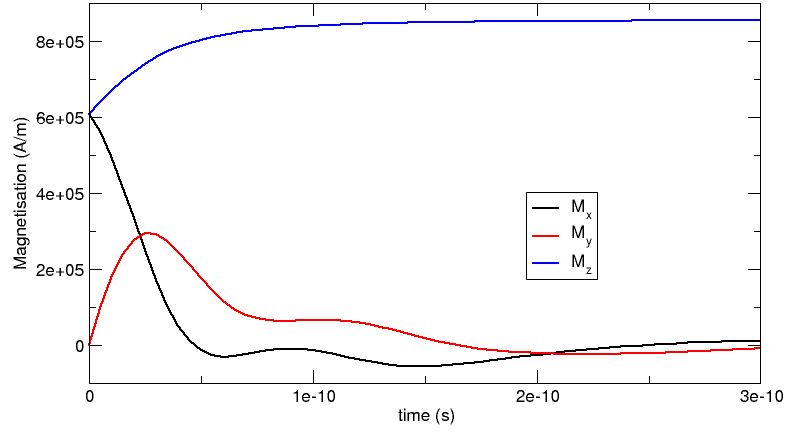
\includegraphics{data_M.png}\hfill}

When we fix the width (here to 15cm), then this is the right size for
pdf, but is poorly rendered in many web browsers (such as mozilla
based family).

{\hfill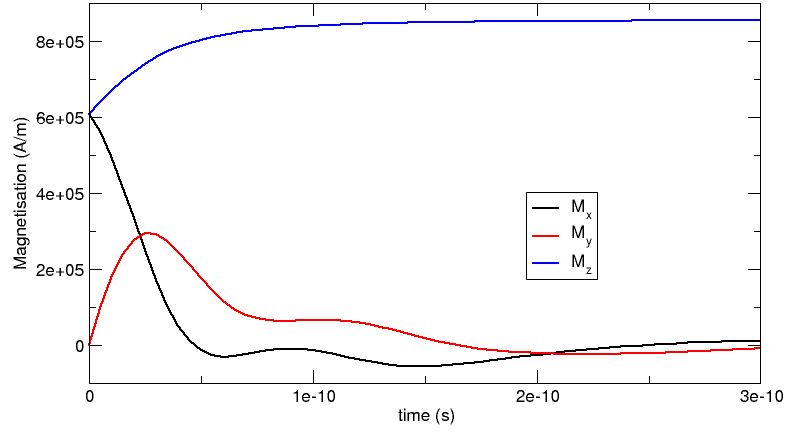
\includegraphics[width=15cm]{data_M.png}\hfill}

The same applies for smaller pictures (equation) where each line
matters (often a minus sign would disappear if the bitmap is scaled
down badly by the browser). This version is great for html (and
happens to be okay in size for the pdf file):

{\hfill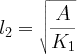
\includegraphics{l_ex_hard.png}\hfill}

Whereas the giving a width provides good results in the pdf file and
poor rendering in the html page (depending on browser, of course).

{\hfill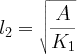
\includegraphics[width=1.5cm]{l_ex_hard.png}\hfill}


%___________________________________________________________________________

\hypertarget{nasty-solution}{}
\pdfbookmark[0]{Nasty solution}{nasty-solution}
\section*{Nasty solution}

We can, of course, use the \texttt{raw} directive to work around this. For
example the following plot will look good on pdf and html:
%

{ \hfill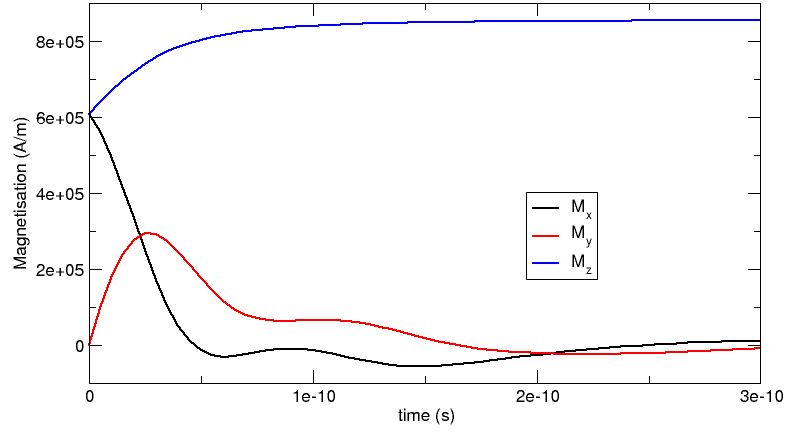
\includegraphics[width=0.9\textwidth]{data_M.png}\hfill}

%
I am not too concerned about the extra effort of adding the same
command twice (if in return the document will realiably have good
looking images and equations!).

However, this is clearly not ideal (because of the duplication of
effort and because of the very specific commands I need to put into
the \texttt{raw} sections).

Could anybody confirm that there is no better way to solve this (at
the moment) or provide suggestions for better alternatives?

Many thanks,

Hans

\begin{center}\small

Generated on: 2007-11-21.
Generated by \href{http://docutils.sourceforge.net/}{Docutils} from \href{http://docutils.sourceforge.net/rst.html}{reStructuredText} source.


\end{center}

\end{document}
